\documentclass[a4paper,12pt]{report}
\usepackage[utf8]{inputenc} % Hỗ trợ mã hóa UTF-8
\usepackage[T1]{fontenc} % Hỗ trợ font tiếng Việt
\usepackage[vietnamese]{babel} % Hỗ trợ ngôn ngữ tiếng Việt
\usepackage{titlesec}
\usepackage{enumitem}
\usepackage{graphicx}
\usepackage{array}
\usepackage{longtable} 

% Tùy chỉnh định dạng cho \part, \chapter, \section, \subsection
\titleformat{\part}{\Huge\bfseries\center}{\thepart}{1em}{}
\titleformat{\chapter}{\Huge\bfseries}{\thechapter}{1em}{}
\titleformat{\section}{\Large\bfseries}{\thesection}{1em}{}
\titleformat{\subsection}{\large\bfseries}{\thesubsection}{1em}{}

\begin{document}

% Trang bìa
\begin{titlepage}
    \centering
    {\LARGE \textbf{TRƯỜNG ĐẠI HỌC SÀI GÒN}} \\[0.2cm]
    {\Large \textbf{KHOA CÔNG NGHỆ THÔNG TIN}} \\[0.5cm]
    
    \vspace{0.5cm} 
    
\includegraphics[width=4cm]{./img/logo.png} % Chèn logo 
    \vspace{0.5cm} % Giảm khoảng cách
    
    {\Large \textbf{HỌC PHẦN: XÂY DỰNG PHẦN MỀM THEO MÔ HÌNH PHÂN LỚP}} \\[0.5cm]
    {\Large Dự án Clone Instagram} \\[0.5cm]

    \vspace{0.5cm} % Giảm khoảng cách
    
    \textbf{Nhóm sinh viên thực hiện:} \\[0.5cm]
    
    \begin{tabular}{|l|l|}
        \hline
        \textbf{Họ và tên} & \textbf{MSSV} \\ \hline
        Văn Tuấn Kiệt & 3122410202 \\ \hline
        Mai Phúc Lâm & 3122410207 \\ \hline
        Nguyễn Đức Duy Lâm & 3122410208 \\ \hline
        Nguyễn Hữu Lộc & 3122410213 \\ \hline
        Hồ Hưng Lộc & 3122410219 \\ \hline
        Vinh & 3122410213 \\ \hline
    \end{tabular}

    \vspace{0.5cm}

    \textbf{Giáo viên hướng dẫn:} Từ Lãng Phiêu \\[0.5cm]
    
    \vfill
    {\Large TP.HCM, 2025}
\end{titlepage}



\newpage

\section*{MỤC LỤC}
\tableofcontents % Tự động tạo mục lục

\newpage

\chapter{Lời cảm ơn}\label{sec:thanks}
\noindent{\large \textbf{LỜI CẢM ƠN}}

\vspace{0.5cm} % Tạo khoảng cách 1cm

Trước hết, chúng em xin gửi lời cảm ơn chân thành đến giảng viên hướng dẫn, người đã tận tình giảng dạy, hỗ trợ và định hướng giúp chúng em hoàn thành dự án này. Những kiến thức mà thầy/cô truyền đạt không chỉ giúp chúng em trong quá trình thực hiện đồ án mà còn là nền tảng quan trọng cho việc phát triển bản thân trong tương lai.

Bên cạnh đó, chúng em xin gửi lời cảm ơn đến gia đình và bạn bè, những người luôn động viên và tạo điều kiện thuận lợi để chúng em có thể tập trung hoàn thành dự án một cách tốt nhất. Sự ủng hộ của mọi người là động lực lớn giúp chúng em vượt qua những khó khăn trong quá trình nghiên cứu và triển khai.

Cuối cùng, chúng em xin cảm ơn các tài liệu tham khảo, cộng đồng lập trình viên, và các diễn đàn công nghệ đã cung cấp nhiều nguồn kiến thức quý giá, giúp chúng em giải quyết những vấn đề gặp phải trong quá trình thực hiện dự án.\\ \\

\chapter{Giới thiệu}\label{sec:introduction}


\vspace{0.5cm} % Tạo khoảng cách 0.5cm

Mạng xã hội ngày nay đóng vai trò quan trọng trong cuộc sống con người, giúp kết nối mọi người trên toàn thế giới, chia sẻ thông tin và tạo ra nhiều giá trị về mặt cá nhân lẫn kinh doanh. Trong số đó, Instagram là một trong những nền tảng nổi bật nhất với hàng triệu người dùng hoạt động mỗi ngày, cung cấp trải nghiệm chia sẻ hình ảnh, video và tương tác trực quan.

Dự án \textbf{Clone Instagram} được xây dựng với mục tiêu mô phỏng lại các tính năng quan trọng của Instagram, bao gồm:
\begin{itemize}
    \renewcommand{\labelitemi}{-} % Thay đổi dấu đầu dòng thành "-"
    \item \textbf{Đăng ký, đăng nhập}: Người dùng có thể tạo tài khoản, đăng nhập và chỉnh sửa thông tin cá nhân.
    \item \textbf{Đăng bài}: Cho phép người dùng đăng tải hình ảnh, viết chú thích và sử dụng hashtag.
    \item \textbf{Thả tim, bình luận}: Người dùng có thể tương tác với bài đăng bằng cách thả tim và để lại bình luận.
    \item \textbf{Nhắn tin}: Hỗ trợ tính năng nhắn tin riêng tư giữa các người dùng.
    \item \textbf{Quản lý hồ sơ cá nhân}: Người dùng có thể xem, chỉnh sửa hồ sơ và theo dõi các hoạt động của mình.
\end{itemize}

Dự án sử dụng \textbf{ReactJS} làm thư viện chính để xây dựng giao diện, kết hợp với \textbf{Firebase} hoặc \textbf{Node.js} để quản lý dữ liệu. Ngoài ra, các thư viện hỗ trợ như \textbf{Redux}, \textbf{React Router}, \textbf{Ant Design}, \textbf{Tailwind CSS} cũng được sử dụng để tối ưu trải nghiệm người dùng và nâng cao hiệu suất ứng dụng.\\ \\

Phân công nhiệm vụ\\

\begin{longtable}{|c|p{12cm}|}
    \hline
    \textbf{Thành viên} & \textbf{Chức năng đã làm} \\
    \hline
    \endfirsthead
    \hline
    \textbf{Thành viên} & \textbf{Chức năng đã làm} \\
    \hline
    \endhead
    \hline
    \endfoot

    Văn Tuấn Kiệt & Nhắn tin, gọi điện, login (backend), AI tạo caption. \\
    \hline
    Nguyễn Đức Duy Lâm & Thống kê, giao diện, bài post, profile. \\
    \hline
    Hồ Hưng Lộc & Profile, thống kê, document. \\
    \hline
    Nguyễn Hữu Lộc & Bài post, thông báo, AI kiểm duyệt nội dung. \\
    \hline
    Mai Phúc Lâm & Bạn bè, chat AI. \\
    \hline
    Quách Hữu Vinh & Comment, tìm kiếm, bảo mật. \\
    \hline
\end{longtable}



\chapter{Lý do chọn đề tài}\label{sec:reason}


\vspace{0.5cm} % Tạo khoảng cách 0.5cm

Mạng xã hội ngày càng phát triển mạnh mẽ, trở thành công cụ không thể thiếu trong đời sống hiện đại. Trong đó, Instagram nổi bật nhờ giao diện tối giản, thân thiện và tích hợp nhiều tính năng hấp dẫn như chia sẻ ảnh, video ngắn, stories, nhắn tin. Với nhu cầu ngày càng cao trong việc phát triển ứng dụng mạng xã hội, việc tìm hiểu và xây dựng một dự án mô phỏng Instagram là cơ hội tốt để sinh viên:

\begin{itemize}
    \renewcommand{\labelitemi}{-} % Thay đổi dấu đầu dòng thành "-"
    \item \textbf{Nâng cao kỹ năng lập trình}: Dự án sử dụng ReactJS giúp sinh viên hiểu rõ hơn về cách phát triển giao diện động, tối ưu hiệu suất và quản lý dữ liệu.
    \item \textbf{Làm quen với kiến trúc ứng dụng hiện đại}: Clone Instagram giúp áp dụng nhiều công nghệ phổ biến như Redux, REST API.
    \item \textbf{Phát triển tư duy UI/UX}: Clone lại Instagram giúp sinh viên học hỏi cách thiết kế giao diện trực quan, thân thiện với người dùng.
    \item \textbf{Ứng dụng thực tế cao}: Sản phẩm có thể mở rộng thêm nhiều tính năng mới, phục vụ học tập hoặc phát triển thành một dự án hoàn chỉnh.
\end{itemize}


\chapter{Yêu cầu chức năng}\label{sec:functional-requirements}
\noindent{\large \textbf{YÊU CẦU CHỨC NĂNG}}

\vspace{0.5cm} % Tạo khoảng cách 0.5cm
\noindent{\normalsize \textbf{Quản lý bài post}}

\begin{itemize}
    \renewcommand{\labelitemi}{-} % Thay đổi dấu đầu dòng thành "-"
    \item \textbf{Thêm bài post}: Đăng tải bài viết kèm hình ảnh, video, văn bản.
    \item \textbf{Chia sẻ bài post}: Thả cảm xúc, hiển thị danh sách bài viết.
    \item \textbf{Bình luận bài post}: Văn bản, emoji, hình ảnh.
\end{itemize}

\vspace{0.3cm}
\noindent{\normalsize \textbf{Quản lý bình luận}}

\begin{itemize}
    \renewcommand{\labelitemi}{-}
    \item \textbf{Thêm comment}: Thả cảm xúc, trả lời comment.
    \item \textbf{Lọc comment}: Theo nội dung, thời gian, người bình luận.
\end{itemize}

\vspace{0.3cm}
\noindent{\normalsize \textbf{Quản lý tin nhắn}}

\begin{itemize}
    \renewcommand{\labelitemi}{-}
    \item \textbf{Gửi tin nhắn}: Văn bản, gọi thoại/video.
    \item \textbf{Hiển thị trạng thái}: Tin nhắn, trạng thái hoạt động.
\end{itemize}

\vspace{0.3cm}
\noindent{\normalsize \textbf{Quản lý hồ sơ cá nhân}}

\begin{itemize}
    \renewcommand{\labelitemi}{-}
    \item \textbf{Chỉnh sửa thông tin}: Cập nhật avatar.
    \item \textbf{Xem danh sách bài post}: Chỉnh sửa bài viết.
\end{itemize}

\vspace{0.3cm}
\noindent{\normalsize \textbf{Quản lý danh sách bạn bè}}

\begin{itemize}
    \renewcommand{\labelitemi}{-}
    \item \textbf{Gửi, hủy, xác nhận}: Lời mời kết bạn.
    \item \textbf{Chặn bạn}: Xem danh sách bạn bè, tìm kiếm bạn bè.
\end{itemize}


\chapter{Yêu cầu phi chức năng}\label{sec:non-functional-requirements}


\begin{itemize}
    \renewcommand{\labelitemi}{-}
    \item \textbf{Hiệu suất}: Tải trang nhanh, tìm kiếm và hiển thị dữ liệu tối ưu.
    \item \textbf{Bảo mật}: Mã hóa dữ liệu, bảo vệ quyền riêng tư, chống tấn công.
    \item \textbf{Trải nghiệm người dùng}: Giao diện thân thiện, điều hướng dễ dàng.
    \item \textbf{Khả năng mở rộng}: Hỗ trợ nhiều người dùng, dữ liệu lớn.
    \item \textbf{Độ tin cậy}: Ổn định, uptime >= 99.9\%.
\end{itemize}



\chapter{Cấu trúc mã nguồn}
\input{chapter/3_CauTRUCMaNguon.tex}

\chapter{Các tính năng được xây dựng}
\noindent{\large \textbf{Các tính năng được xây dựng}}


\vspace{0.5cm} % Tạo khoảng cách 0.5cm
\noindent{\normalsize \textbf{Quản lý bài post}}
\begin{itemize}
    \renewcommand{\labelitemi}{-} % Thay đổi dấu đầu dòng thành "-"
    \item \textbf{Thêm bài post:} Đăng tải bài viết kèm hình ảnh, video, văn bản. Hình ảnh và video được upload lên Cloudinary thông qua API \texttt{POST /api/post}.
    \item \textbf{Chia sẻ bài post:} Thả cảm xúc (like), hiển thị danh sách bài viết, chia sẻ bài post.
    \item \textbf{Bình luận bài post:} Hỗ trợ văn bản, emoji (dùng \texttt{@emoji-mart/react}), và hình ảnh (tích hợp Cloudinary).
    \item \textbf{Xóa bài post:} Người dùng có thể xóa bài post của mình thông qua API \texttt{DELETE /api/post/\{id\}}.
\end{itemize}

\vspace{0.3cm}
\noindent{\normalsize \textbf{Quản lý bình luận}}
\begin{itemize}
    \renewcommand{\labelitemi}{-}
    \item \textbf{Thêm comment:} Thả cảm xúc (like), trả lời comment (hỗ trợ comment lồng nhau).
    \item \textbf{Lọc comment:} Theo nội dung, thời gian, hoặc người bình luận, giúp người dùng dễ dàng tìm kiếm bình luận.
    \item \textbf{Xóa comment:} Người dùng có thể xóa bình luận của mình hoặc của người khác (nếu là chủ bài post).
\end{itemize}

\vspace{0.3cm}
\noindent{\normalsize \textbf{Quản lý tin nhắn}}
\begin{itemize}
    \renewcommand{\labelitemi}{-}
    \item \textbf{Gửi tin nhắn:} Hỗ trợ văn bản, hình ảnh.
    \item \textbf{Hiển thị trạng thái:} Hiển thị trạng thái tin nhắn (đã gửi, đã xem), trạng thái hoạt động của người dùng (online/offline).
    \item \textbf{Tạo nhóm chat:} Hỗ trợ tạo nhóm chat với tối đa 100 người, tích hợp với module \texttt{Friends} để thêm thành viên.
\end{itemize}

\vspace{0.3cm}
\noindent{\normalsize \textbf{Quản lý hồ sơ cá nhân}}
\begin{itemize}
    \renewcommand{\labelitemi}{-}
    \item \textbf{Chỉnh sửa thông tin:} Cập nhật avatar (upload lên AWS S3), chỉnh sửa thông tin như tên, email, mô tả.
    \item \textbf{Xem danh sách bài post:} Hiển thị tất cả bài post của người dùng, cho phép chỉnh sửa hoặc xóa bài viết.
    \item \textbf{Xem thông tin công khai:} Hiển thị thông tin hồ sơ (avatar, số lượng bài post, số lượng bạn bè) cho người dùng khác xem.
\end{itemize}

\vspace{0.3cm}
\noindent{\normalsize \textbf{Quản lý danh sách bạn bè}}
\begin{itemize}
    \renewcommand{\labelitemi}{-}
    \item \textbf{Gửi, hủy, xác nhận:} Gửi lời mời kết bạn, hủy lời mời, hoặc xác nhận lời mời từ người khác. Khi xác nhận, hệ thống tự động tạo cuộc trò chuyện (tích hợp với module \texttt{Message}).
    \item \textbf{Chặn bạn:} Chặn người dùng, xem danh sách bạn bè, tìm kiếm bạn bè theo tên hoặc email.
\end{itemize}

\vspace{0.3cm}
\noindent{\normalsize \textbf{Quản lý thông báo}}
\begin{itemize}
    \renewcommand{\labelitemi}{-}
    \item \textbf{Gửi thông báo thời gian thực:} Thông báo khi có lời mời kết bạn, bình luận mới, hoặc tin nhắn mới, sử dụng WebSocket và RabbitMQ để xử lý bất đồng bộ.
    \item \textbf{Hiển thị danh sách thông báo:} Hiển thị tất cả thông báo của người dùng, cho phép đánh dấu đã đọc hoặc xóa thông báo.
\end{itemize}

\vspace{0.3cm}
\noindent{\normalsize \textbf{Tìm kiếm}}
\begin{itemize}
    \renewcommand{\labelitemi}{-}
    \item \textbf{Tìm kiếm người dùng:} Tìm kiếm người dùng theo tên hoặc email, hiển thị danh sách kết quả.
    \item \textbf{Tìm kiếm bài post:} Tìm kiếm bài post theo nội dung hoặc hashtag.
   
\end{itemize}



\chapter{Sơ đồ ERD}

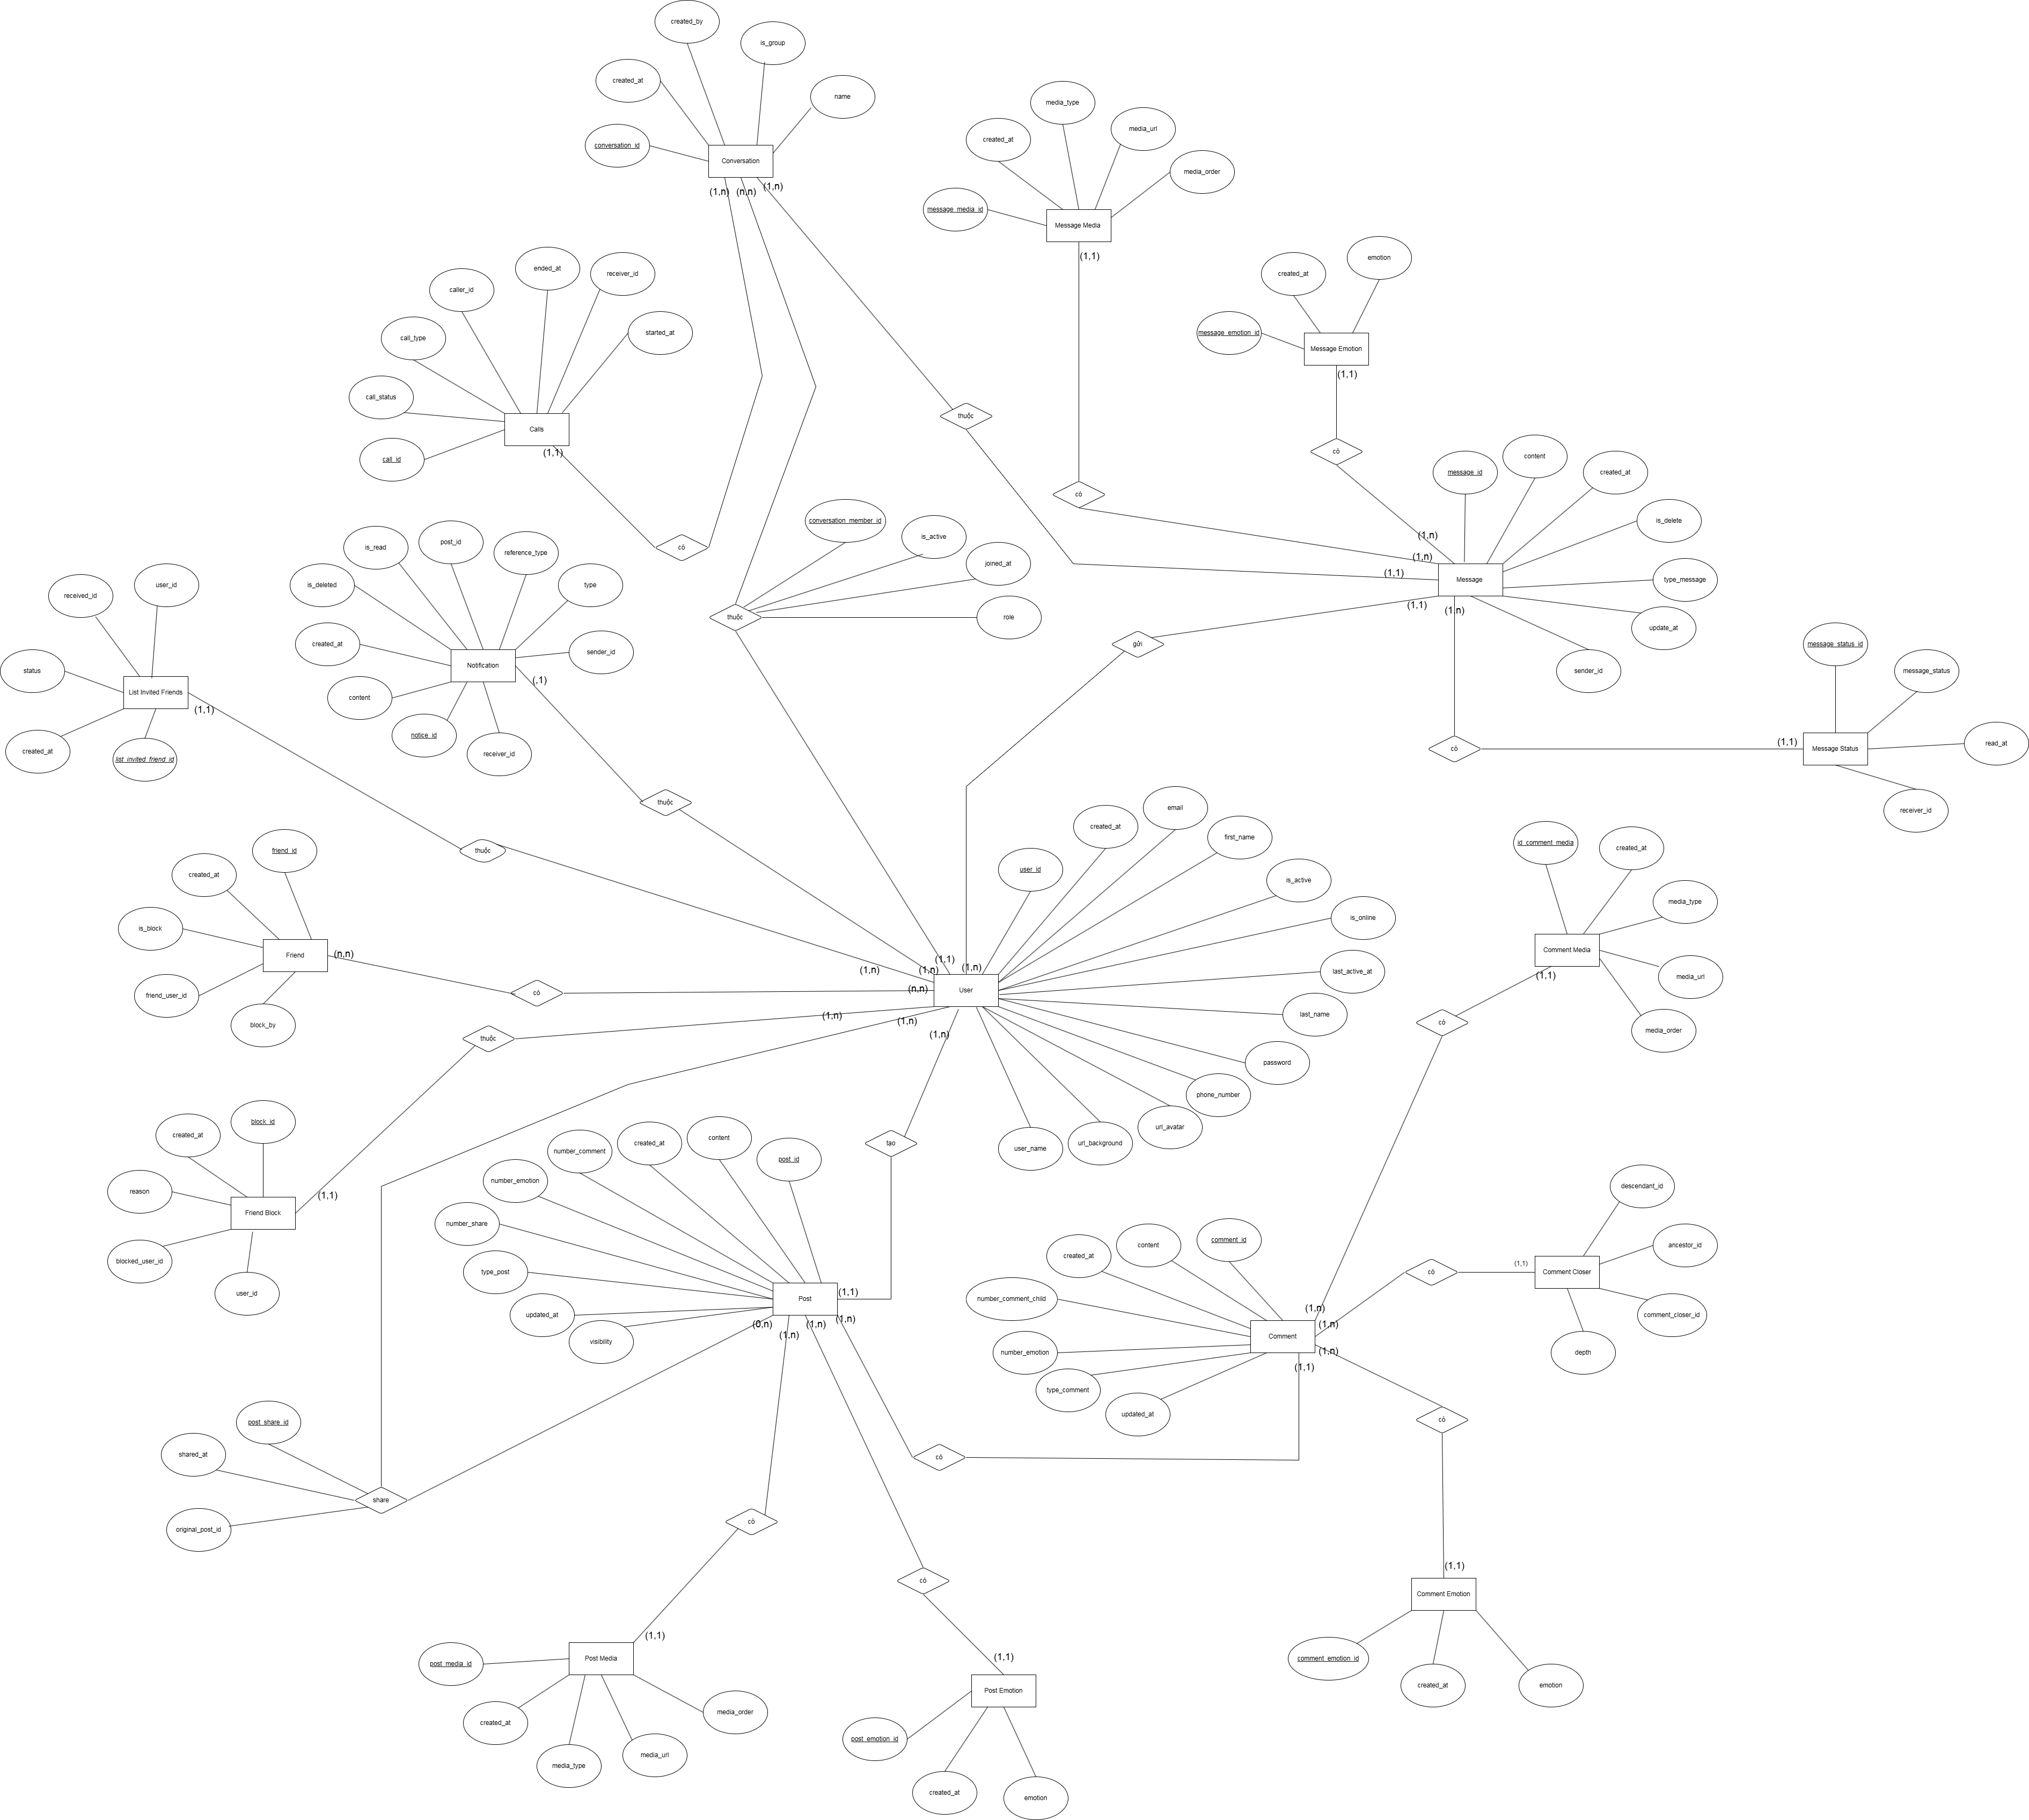
\includegraphics[width=\textwidth]{img/ERD_Instagram}


\end{document}